\documentclass[letterpaper,12pt,fleqn]{article}
\usepackage{matharticle}
\usepackage{graphtheory}
\pagestyle{empty}
\begin{document}

\section*{Graph Operations}

\begin{enumerate}[left=0pt]
\item Union

  \begin{definition}[Union]
    Let \(G\) and \(H\) be two disjoint graphs.  The \emph{union} of \(G\) and \(H\), denoted by \(G\cup H\), is
    the disconnected graph such that:
    \begin{gather*}
      V(G\cup H)=V(G)\cup V(H) \\
      E(G\cup H)=E(G)\cup E(H)
    \end{gather*}
    When \(G=H\), the alternate notation \(2G\) can be used.
  \end{definition}

  \begin{example}
    Let \(G_1=G_2=P_2\), \(G_4=C_4\), and \(G_4=K_5\):

    \bigskip

    \begin{center}
      \begin{tikzpicture}[every node/.style={unlabeled node}]
        \pathN{2}{(0,-0.5)}{above}{};
        \pathN{2}{(1,-0.5)}{above}{};
        \cycleN{4}{(3,0)}{0.5in}{135}{}
        \completeN{5}{(6,0)}{0.5in}{0}{}
      \end{tikzpicture}

      \(G=2P_2\cup C_4\cup K_5\)
    \end{center}
  \end{example}

\item Join

  \begin{definition}[Join]
    Let \(G\) and \(H\) be two disjoint graphs.  The \emph{join} of \(G\) and \(H\), denoted \(G+H\), is the
    graph such that:
    \begin{gather*}
      V(G+H)=V(G)\cup V(H) \\
      E(G+H)=E(G)\cup E(H)\cup\setb{uv}{u\in G\ \text{and}\ v\in H}
    \end{gather*}
  \end{definition}

  \begin{example}
    Let \(G_1=P_2\) and \(G_2=P_4\):
    \begin{center}
      \begin{tikzpicture}[every node/.style={unlabeled node},node distance=1cm]
        \pathN{2}{(0,0)}{above}{l};
        \pathN{4}{(2,-1.25cm)}{above}{r};
        \foreach \i in {1,2}{
          \foreach \j in {1,2,3,4}{
            \draw (l\i) edge (r\j);
          }
        }
      \end{tikzpicture}

      \(G=P_2+P_4\)
    \end{center}
  \end{example}

\item Product

  \begin{definition}[Product]
    Let \(G\) and \(H\) be two disjoint graphs.  The \emph{product} of \(G\) and \(H\), denoted \(G\times H\), is
    the graph such that:
    \begin{gather*}
      V(G\times H)=V(G)\times V(H) \\
      E(G\times H)=\setb{\set{(u,v),(x,y)}}{u=x\ \text{and}\ vy\in E(H)\ \text{or}\ v=y\ \text{and}\ ux\in E(G)}
    \end{gather*}
  \end{definition}

  \begin{example}
    \begin{minipage}{1.5in}
      \begin{center}
        
\begin{tikzpicture}[every node/.style={labeled node}]
          \cycleV{\(1\),\(2\),\(3\)}{(0,0)}{0.5in}{90}{};
        \end{tikzpicture}

        \bigskip

        \(C_3\)
      \end{center}
    \end{minipage}
    \begin{minipage}{1.5in}
      \begin{center}
        \begin{tikzpicture}[every node/.style={labeled node},node distance=0.75in]
          \pathV{\(4\),\(5\)}{(3,0)}{right}{}
        \end{tikzpicture}

        \bigskip

        \(P_2\)
      \end{center}
    \end{minipage}
    \begin{minipage}{3in}
      \begin{center}
        \begin{tikzpicture}[every node/.style={labeled node}]
          \cycleV{{\((1,4)\)},{\((2,4)\)},{\((3,4)\)}}{(0,6)}{0.75in}{180}{t}
          \cycleV{{\((1,5)\)},{\((3,5)\)},{\((2,5)\)}}{(0,0)}{0.75in}{180}{b}
          \draw (t1) edge (b1);
          \draw (t3) edge (b2);
          \draw (t2) -- ($(t2) + (1.5cm,0)$) |- (b3);
        \end{tikzpicture}

        \bigskip
        
        \(G=C_3\times P_2\)
      \end{center}
    \end{minipage}
  \end{example}
  
\item Complement
  
  \begin{definition}[Complement]
    Let \(G\) be a graph.  The \emph{complement} of \(G\), denoted by \(\comp{G}\), is the graph:
    \begin{gather*}
      V(\comp{G})=V(G) \\
      E(\comp{G})=\ps_2\left(V(G)\right)-E(G)
    \end{gather*}
    In other words, \(\forall\,u,v\in V(\comp{G}),uv\in E(\comp{G})\iff uv\notin (G)\).
  \end{definition}

  \begin{example}
    \begin{minipage}{2in}
      \begin{center}
        \begin{tikzpicture}[every node/.style={unlabeled node}]
          \cycleNnodes{4}{(0,0)}{0.5in}{135}{}
          \draw (1) edge (2) edge (3) edge (4);
          \draw (3) edge (4);
          \draw [dotted,red] (2) edge (3) edge (4);
        \end{tikzpicture}

        \bigskip

        \(G\)
      \end{center}
    \end{minipage}
    \begin{minipage}{2in}
      \begin{center}
        \begin{tikzpicture}[every node/.style={unlabeled node}]
          \cycleNnodes{4}{(0,0)}{0.5in}{135}{}
          \draw [dotted,red] (1) edge (2) edge (3) edge (4);
          \draw [dotted,red] (3) edge (4);
          \draw (2) edge (3) edge (4);
        \end{tikzpicture}

        \bigskip

        \(\comp{G}\)
      \end{center}
    \end{minipage}
  \end{example}

\end{enumerate}

\begin{theorem}
  Let \(G\) be a graph:
  \begin{quote}
    \(G\) is disconnected \(\implies\comp{G}\) is connected and \(\diam(\comp{G})\le2\).
  \end{quote}
\end{theorem}

\begin{proof}
  Assume \(G\) is disconnected.

  Thus, \(G\) contains two or more components.  Now assume \(u,v\in V(G)\) and so \(u,v\in V(\comp{G})\).
  \begin{description}
  \item[Case 1:] \(uv\notin E(G)\)

    \(\therefore uv\in E(\comp{G})\) and \(d_{\comp{G}}(u,v)=1\).
      
    \item[Case 2:] \(uv\in E(G)\)

      This means that \(u\) and \(v\) are in the same component in \(G\).  Furthermore, \(uv\notin E(\comp{G})\).
      However, since \(G\) is disconnected, there exists a distinct vertex \(w\) in a different component in \(G\),
      and so \(uw,vw\in E(\comp{G})\).  Consider the path \((u,w,v)\).  This is a \(u-v\) path in \(\comp{G}\) of
      length \(2\).

      \(\therefore u\) and \(v\) are connected and \(d_{\comp{G}}(u,v)=2\).
  \end{description}

  \(\therefore u\) and \(v\) are connected in \(\comp{G}\) and \(\diam(\comp{G})\le2\).
\end{proof}

\end{document}
